\documentclass[a4paper, fontsize=14pt]{article}
\usepackage{scrextend}
\usepackage{indentfirst, fancyhdr, amsfonts, mathtools, amssymb}
\usepackage{titlesec} %работа с рубрикацией
\usepackage{tocloft} %настройки оглавления
\usepackage[T2A]{fontenc}
\usepackage[utf8x]{inputenc}
\usepackage[russian]{babel}
\usepackage{hyperref} %кликабельное оглавление
\usepackage[left=3.7cm,right=2cm,top=2cm,bottom=2cm]{geometry}
\usepackage{tempora} %настраиваем шрифт типа TNR                                   
\usepackage{newtxmath} %делаем шрифт формул похожим на TNR
\usepackage{caption}
\usepackage{listings}
\usepackage{pdfpages}
\lstset{
  columns=fullflexible,
  breaklines=true,
}
\linespread{1}
\setcounter{page}{4} %в зависимости от того, какой по счёту страницей должно быть оглавление!

%НАСТРОЙКИ ОГЛАВЛЕНИЯ
\renewcommand{\cftsecaftersnum}{.} %точки после номеров разделов и подразделов в оглавлении
\renewcommand{\cftsubsecaftersnum}{.}
\renewcommand{\cftsecfont}{\normalfont} %разделы в оглавлении пишутся обычным (не жирным) шрифтом
\renewcommand{\cftsecpagefont}{\normalfont} %соответствующие им страницы тоже
\renewcommand{\cftsecleader}{\cftdotfill{\cftdotsep}} %расставляем точки между названиями разделов и их страницами
\addto\captionsrussian{\renewcommand\contentsname{СОДЕРЖАНИЕ}} %хотим, чтобы слово "Содержание" писалось капсом
\renewcommand{\cfttoctitlefont}{\hfil\bfseries} %слово СОДЕРЖАНИЕ по центру жирным
\renewcommand{\cftaftertoctitle}{\hfill}

%НАСТРОЙКИ РУБРИКАЦИИ
\titleformat*{\section}{\center\bf} %названия разделов и подразделов по середине жирным шрифтом
\titleformat*{\subsection}{\center\bf}
\titlelabel{\thetitle.\quad} %название раздела и его номер отделены точкой

%НАСТРОЙКИ БИБЛИОГРАФИИ
\addto\captionsrussian{\renewcommand\refname{СПИСОК ЛИТЕРАТУРЫ}} %хотим, чтобы слова "Список литературы" писались капсом
\makeatletter
\renewcommand{\@biblabel}[1]{#1.} %хотим, чтобы в списке литературы номера источников писались в формате "No. <...>", а не "[No] <...>"
\makeatother

\begin{document}
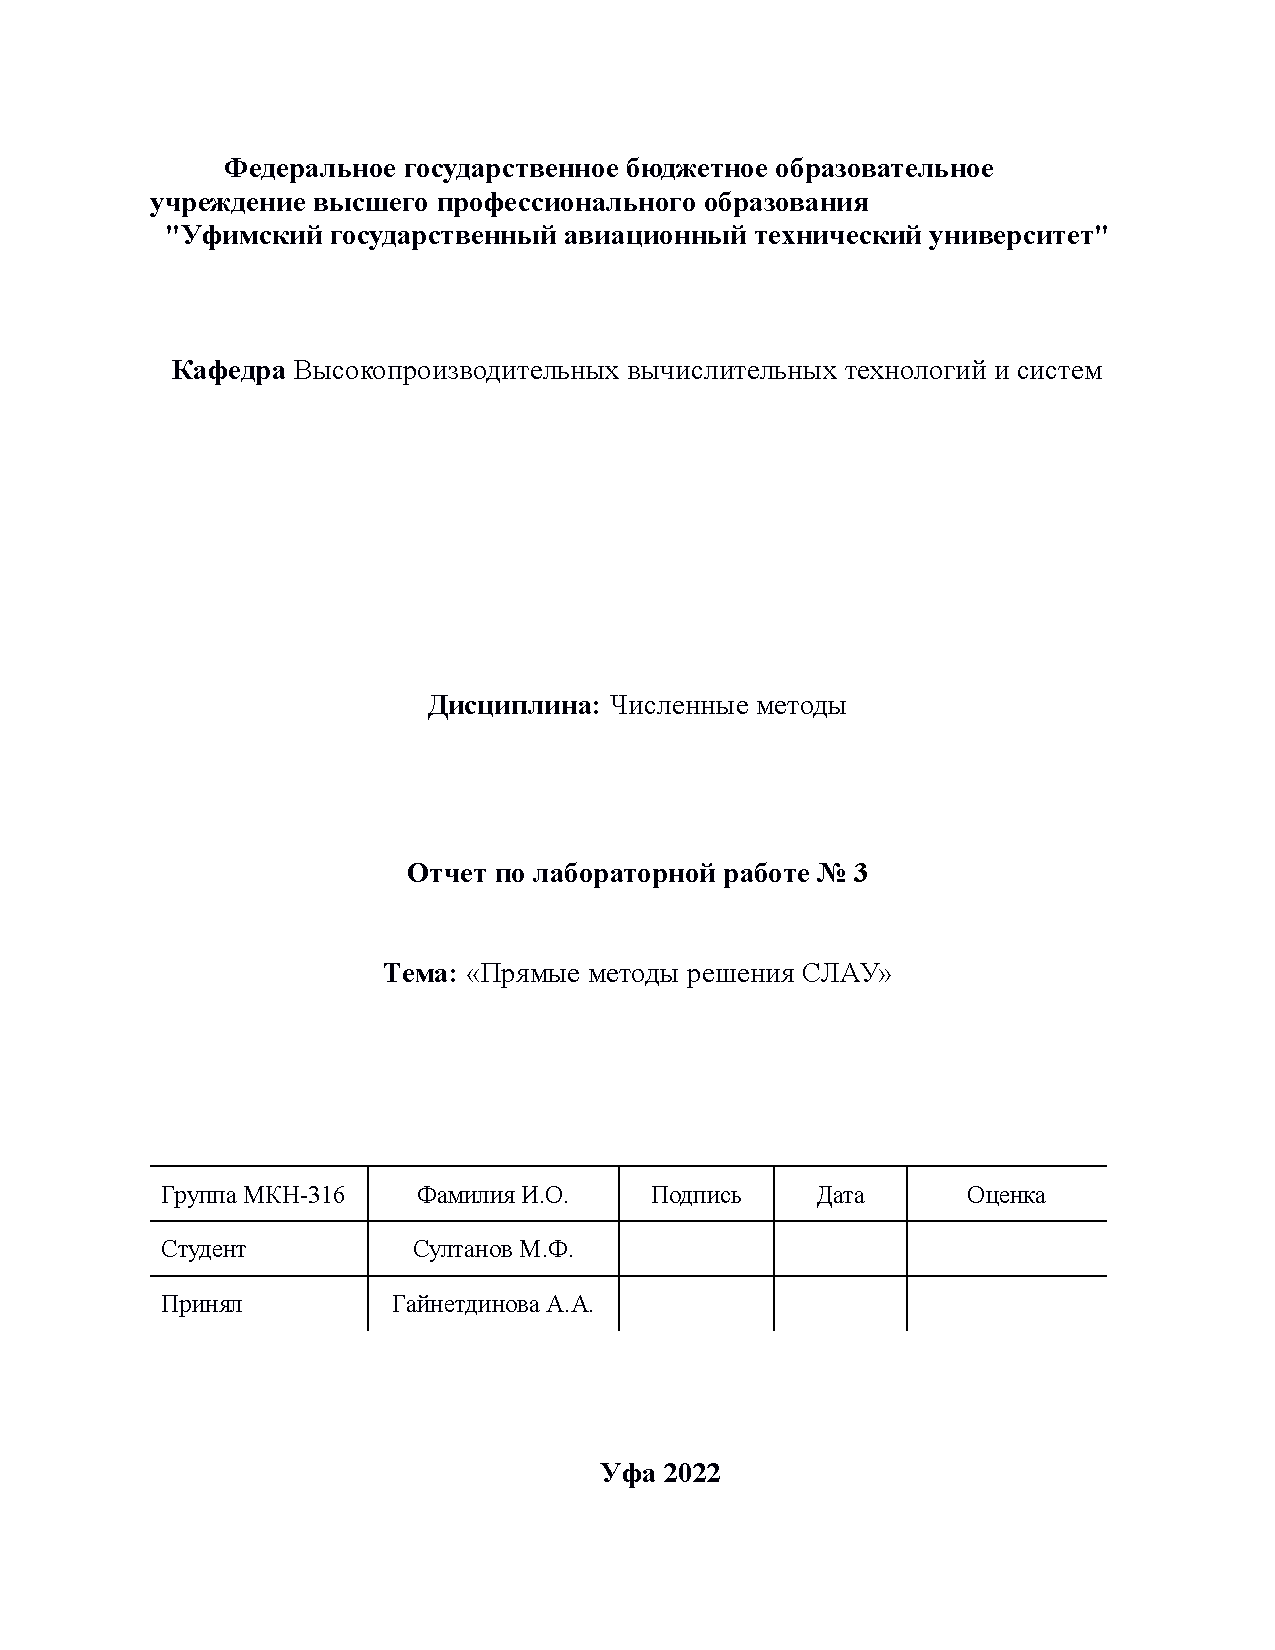
\includepdf[pages={1}]{src/front_page.pdf}
\textbf{Цель работы:} получить навык численного решения систем линейных алгебраических уравнений (СЛАУ) с использованием различных прямых методов.
\subsection*{{Ход работы}}
\subsubsection*{Задача №1}
\begin{enumerate}
    \item Написать вычислительную программу на языке программирования C++ для решения СЛАУ методом Гаусса с выбором ведущего элемента.
    \item С использованием написанной программы решить задачу о
    рациональной интерполяции: выполнить приближение функции $y(x)$,
    заданной таблично, рациональной функцией вида
    
    \begin{equation}
        \label{rational_interp}
        f(x) = \frac{P(x)}{Q_(x)}, \quad \operatorname{deg} P(x) \leq \operatorname{deg} Q(x) 
    \end{equation}
    При этом требуется определить значения $p = \operatorname{deg} P(x)$ и $q = \operatorname{deg} Q(x)$
    \item Построить график интерполирующей функции и исходных данных.
\end{enumerate}
\subsubsection*{Решение}
    Метод Гаусса решения СЛАУ $Ax = b$ состоит из двух этапов:

\textbf{1 этап: } прямой ход ~-- приведение системы элементарными преобразованиями строк к треугольному виду (сверху вниз) с едининчными диагональными элементами.

\textbf{2 этап: } обратный ход ~-- вычисление координат решения (снизу вверх)

\begin{equation*}
    x_i =b_i - \sum_{j = i+1}^{n-1} a_{ij} x_j, \quad i = n-1, \dots, 0
\end{equation*}

В ходе программной реализации по описанному алгоритму нельзя проводить исключения, если в ходе расчета на
главной диагонали оказался нулевой элемент или элемент, достаточно близкий к
нулю. Чтобы избежать этого каждый цикл всегда начинают с перестановки строк.
Среди элементов столбца $a_{ij}, i \geq j$ находят главный, т.е. наибольший по модулю
в текущем столбце, и перестановкой строк переводят его на главную диагональ,
после чего делают исключения.

Приложением метода Гаусса является решение системы, появляющейся в ходе рациональной интерполяции. Пусть задана табличная функция с $n = 6$ точками \eqref{eq:table_func}.

\begin{equation}
    \label{eq:table_func}
    \begin{aligned}
        f(x) = \{&(-2.25,0.29422), &(-1.65, 0.18737), \\
                &(-1.05, -1.0215), &(-0.45,-5.4471), \\
                &(-1.4440,0.15), &(2.5873, 0.75)\}
        \end{aligned}
\end{equation}

Необходимо построить интерполяционный многочлен в виде \eqref{rational_interp}.
Пусть $\operatorname{deg} P = p, \operatorname{deg} Q = q, p + q + 1= n, q > p$. Тогда \eqref{rational_interp} с условием интерполяции можно переписать в виде:
\begin{equation*}
    \frac{a_0 + a_1 x_i + \dots + a_p x_i^p}{b_0 + b_1 x_i + \dots b_q x^q} = y_i
\end{equation*}

Домножим обе части на знаменатель:
\begin{equation*}
    a_0 + a_1 x_i + \dots + a_p x_i^p = y_i (b_0 + b_1 x_i + \dots b_q x^q)
\end{equation*}

Многчлен $P(x)$ дает $p+1$ неизвестный коэффициент, многочлен $Q(x)$ дает $q + 1$ неизвестный коэффициент. Получаем $n$ уравнений с  $n+1$ неизвестными.
Пложим $b_0 = 1$ и получим СЛАУ:
\begin{equation*}
    a_0 + a_1 x_i + \dots a_{p} x_i^p - b_1 y_i x_i - \dots - b_{n-   1-p} y_i x_i^{n-1-p} = y_i, \quad i = 0 \dots n - 1
\end{equation*}

Пусть $p = 1, q = 4$, тогда полученная СЛАУ примет вид:
\begin{equation*}
    \begin{pmatrix}
        1.00&  -2.25&   0.66&  -1.49&   3.35&  -7.54& \\
        1.00&  -1.65&   0.31&  -0.51&   0.84&  -1.39& \\
        1.00&  -1.05&  -1.07&   1.13&  -1.18&   1.24& \\
        1.00&  -0.45&  -2.45&   1.10&  -0.50&   0.22& \\
        1.00&  -2.25&   0.66&  -1.49&   3.35&  -7.54& \\ 
        1.00&  -1.65&   0.31&  -0.51&   0.84&  -1.39& \\           
        1.00&  -1.05&  -1.07&   1.13&  -1.18&   1.24& \\           
        1.00&  -0.45&  -2.45&   1.10&  -0.50&   0.22& \\                    
        1.00&   0.15&   0.22&   0.03&   0.00&   0.00& \\                                   
        1.00&   0.75&  -1.94&  -1.46&  -1.09&  -0.82&
    \end{pmatrix}
    \begin{pmatrix}
        a_0 \\
        a_1 \\
        b_1 \\
        b_2 \\
        b_3 \\
        b_4 
    \end{pmatrix}   
    =
    \begin{pmatrix}
        0.29\\  0.19\\ -1.02\\ -5.45\\ -1.44\\  2.59\\
    \end{pmatrix}      
\end{equation*}

Решим её методом Гаусса, получим:
\begin{equation*}
    \begin{pmatrix}
        a_0 \\
        a_1 \\
        b_1 \\
        b_2 \\
        b_3 \\
        b_4 
    \end{pmatrix} =
    \begin{pmatrix}
        &-1.52\\ &-1.19\\  &1.59\\ &-2.04\\ &-3.88\\ &-1.07\\
    \end{pmatrix} 
\end{equation*}

Таким образом 
\begin{equation}
    \label{eq:p1q4}
    f(x) = \frac{P(x)}{Q(x)} = \frac{-1.52 -1.19x}{1 + 1.59x -2.04x^2 -3.88x^3 -1.07x^4}
\end{equation}

Аналогично поступим при $p = 2, q = 3$. Получим функцию
\begin{equation}
    \label{eq:p2q3}
    f(x) = \frac{P(x)}{Q(x)} = \frac{-2.09 +  2.33x + 2.70x^2}{1 +  1.27x -0.85x^2 -2.42x^3}
\end{equation}
Графики функции \eqref{eq:p1q4} и \eqref{eq:p2q3} представлены на рисунках 1 и 2. Точками обозначены данные табличной функции \eqref{eq:table_func}.

\begin{center}
    \label{p1q4}
        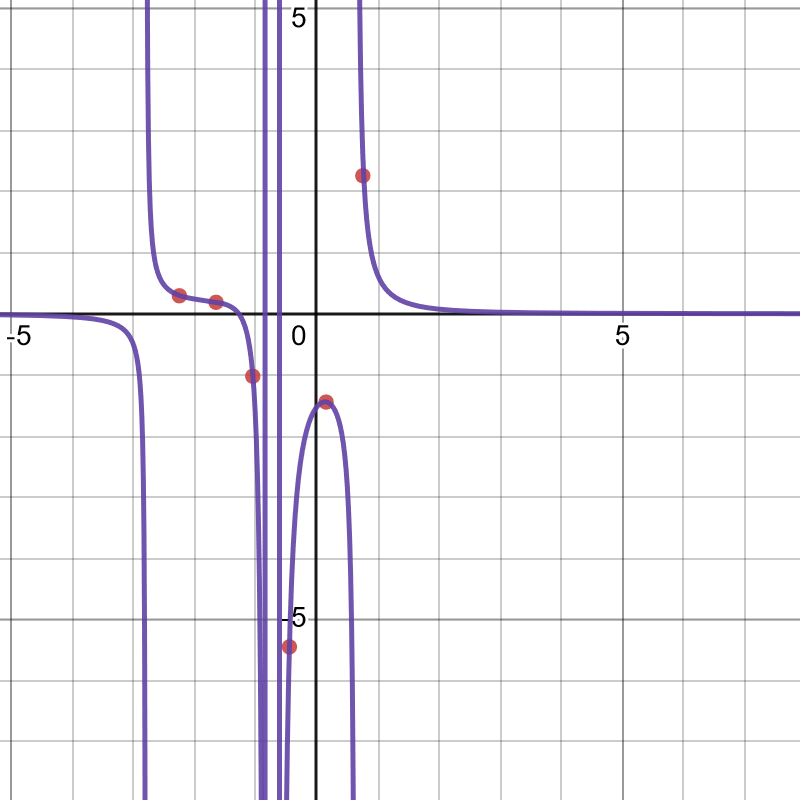
\includegraphics[scale=0.3]{src/p1q4}
    \captionof{figure}{График рационального интерполирования при $p=1, q = 4$}
\end{center}

\begin{center}
    \label{p2q3}
        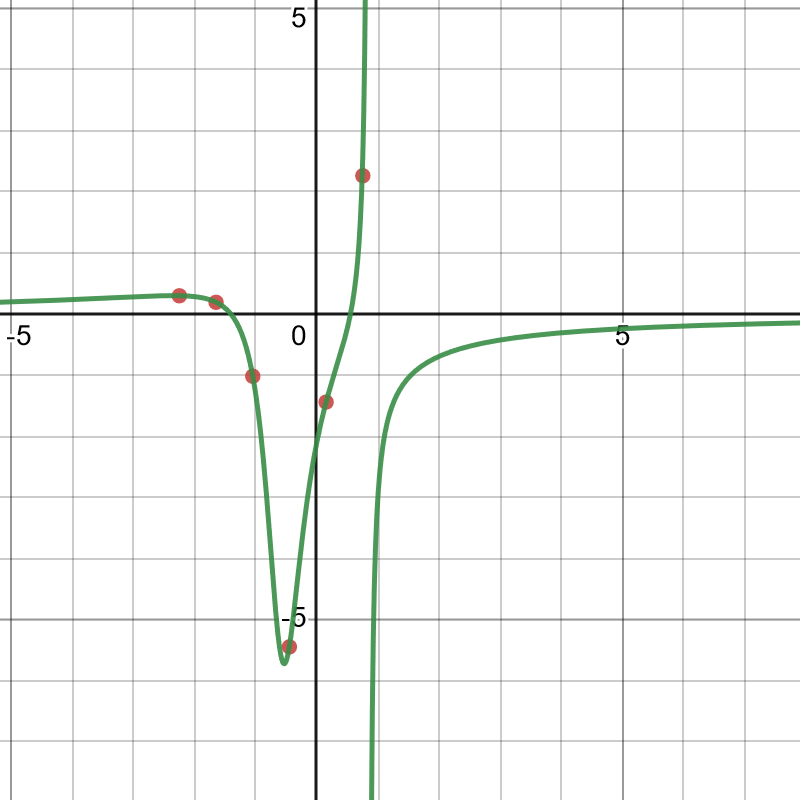
\includegraphics[scale=0.3]{src/p2q3}
    \captionof{figure}{График рационального интерполирования при $p=2, q = 3$}
\end{center}    

Таким образом, наиболее оптимальным образом табличную функцию \eqref{eq:table_func} приближает рациональная интерполяция, заданная формулой \eqref{eq:p2q3}.

\subsubsection*{Задача №2}
\begin{enumerate}
    \item Написать вычислительную программу на языке программирования C++
    для решения СЛАУ методом LU-разложения
    \item Выполнить п. 2, п. 3 задачи 1
\end{enumerate}
\subsubsection*{Решение}
$LU$-разложение ~-- это представление матрицы $A_{n\times n}$ в виде произведения двух матриц, $A = LU$, где $L$ нижняя треугольная матрица, $U$ верхняя треугольная матрица сединичной диагональю.
Пусть дана СЛАУ и главные миноры матрицы $A$ ненулевые. Элементы $l_{ij}$ и $u_{ij}$ определяются из условия:
\begin{equation*}
    \sum_{k=1}^{n} l_{ik} u_{kj} = a_{ij}, \quad i,j = 1, \dots, n
\end{equation*}
Тогда их можно получить по формулам:
\begin{equation*}
    l_{i1} = a_{i1}, \quad u_{1j} = \frac{a_{1j}}{l_{11}} \quad 1 < i \leq j
\end{equation*}
\begin{equation*}
    u_{ij} = a_{ij} - \sum_{k=1}^i l_{ik} u_{kj} \quad 1 < i \leq j
\end{equation*}
\begin{equation*}
    l_{ji} = \frac{1}{u_{ii}} \left(a_{ji} - \sum_{k=1}^i l_{jk} u_{ki}\right)
\end{equation*}
Затем система может быть представлена в виде двух СЛАУ с треугольными матрицами:
\begin{equation*}
    Ax = d \Rightarrow LUx = d \Rightarrow 
    \begin{cases}
        Ux = y \\
        Ly = d
    \end{cases}
\end{equation*}

Решаются обе системы подобно обратному ходу метода Гаусса. 

При решении задачи рациональной интерполяции метод Гаусса и $LU$-разложение дают одинаковый результат.

$LU$-разложение требует примерно $\frac{2 n^3}{3}$ операций, а колличество операций для вычисления нижне- и верхнетреугольных матриц пропорционально $n$.
Таким образом, главное преимущество метода LU-разложения заключается в том,
что явный вид вектора правой части $b$ при решении СЛАУ
используется только на заключительном этапе (в формулах
прямого хода), а наиболее трудоемкие операции по вычислению
самих матриц $L$ и $U$ вовсе не требуют знания вектора $b$. Таким
образом, если решается серия СЛАУ с одной и той же матрицей
$A$, но разными правыми частями $b$, то очень
выгодно единожды вычислить $LU$-разложение матрицы $A$, а уже
затем быстрой подстановкой решить каждую из конкретных
систем.
\subsubsection*{Задача №3}
\begin{enumerate}
    \item Написать вычислительную программу на языке программирования C++
    для решения СЛАУ с симметричной матрицей методом квадратного
    корня.
    \item С использованием написанной программы решить задачу об
    аппроксимации функции из первой лабораторной работы, заданной на
    равномерной сетке из 20 узлов, многочленами степени $1 \leq n \leq 11$ с
    использованием метода наименьших квадратов.
    \item Построить графики аппроксимирующих многочленов и исходных
    данных.
    \item Определить степень многочлена, обеспечивающего наилучшее
    приближение (соответствующее наименьшему значению суммы
    квадратов отклонений значений многочлена в узлах сетки от исходных
    данных)
\end{enumerate}
\subsubsection*{Решение}
Разложение Холецкого — представление симметричной положительно определённой матрицы матрицы в виде:
\begin{equation*}
    A = L L^T
\end{equation*}
где $L$ ~-- это нижняя треугольная матрица (нули сверху от
диагонали), а транспонированная матрица $L^T$ является верхней
треугольной. 

Однако удобно искать матрицу $L$ по формулам:
\begin{equation*}
    l_{ii} = \sqrt{a_{ii} - \sum_{k=1}^{i-1} l^2_{ik}}, \quad l_{ij} = \frac{1}{l_{jj}} \left( a_{ij} - \sum_{k=1}^{j-1} l_{ik} l_{jk}\right) \quad j < i
\end{equation*}

Метод наименьших квадратов ~-- метод аппроксимации основанный на минимизации суммы квадратов отклонений некоторых функций от экспериментальных входных данных. 
Пусть заданы данные $\{ x_i, y_i\}, i = 1 \dots n$. Будем искать линейную аппроксимацию в виде $\tilde{y}_m = a_0 + a_1 x + \cdots + a_m x^m$. Тогда,
\begin{equation*}
    R^2 = \sum_{i=1}^n \biggr[ y_i - \bigr(a_0 + a_1 x_i + \cdots + a_m x_i^m\bigr)\biggr]^2
\end{equation*}

Необходимо минимизировать $R^2$, таким образом, нужно найти
\begin{equation*}
    \min_x || Xa - y ||^2
\end{equation*}

То есть линейная задача наименьших квадратов заключается
в нахождении такого вектора $a$, называемого псевдорешением
системы $Xa = y$, на котором достигается минимум.

Доказывается, что множество псевдорешений системы $Xa = y$ совпадает с множеством решений системы:

\begin{equation}
    \label{eq:pseudo_sol}
    X^T X a = X^T y
\end{equation}

Матрица $X^T X$ является симметрической и её можно разложить по методу Холецкого.

По заданию исходной функцией являлась $f(x) = \frac{\operatorname{arctan}(x)}{1 + x^2}$. По ней была получена следующая таблица данных на равномерной сетке:
\begin{equation}
    \label{eq:sqr_data}
    \begin{matrix}
        (0.00,0.00),(0.10,0.09),(0.19,0.18),(0.29,0.26)&\\
        (0.38,0.32),(0.48,0.36),(0.57,0.39),(0.67,0.41)&\\
        (0.76,0.41),(0.86,0.41),(0.95,0.40),(1.05,0.39)&\\
        (1.14,0.37),(1.24,0.35),(1.33,0.33),(1.43,0.32)&\\
        (1.52,0.30),(1.62,0.28),(1.71,0.26),(1.81,0.25)&
    \end{matrix}
\end{equation}

Подставив данные \eqref{eq:sqr_data} в уравнение \eqref{eq:pseudo_sol} получим решение (наилучшее при $n=11$):
\begin{equation}
    \label{eq:sqr_sol}
    \begin{aligned}
        \tilde{y} = &1.001159x^{1}-0.028163x^{2}-1.070042x^{3} -\\
        &-1.279338x^{4}+5.134843x^{5}-5.992231x^{6} +\\
        &+3.674453x^{7} -1.229696x^{8}+0.177546x^{9} +\\
        &+ 0.008222x^{10}-0.004054x^{11}
    \end{aligned}
\end{equation}

Погрешность в худшем случае при этом составляет около $3 \cdot 10^{-6}$. График многочлена \eqref{eq:sqr_sol}приведен на рисунке 3.
\begin{center}
    \label{p1q4}
        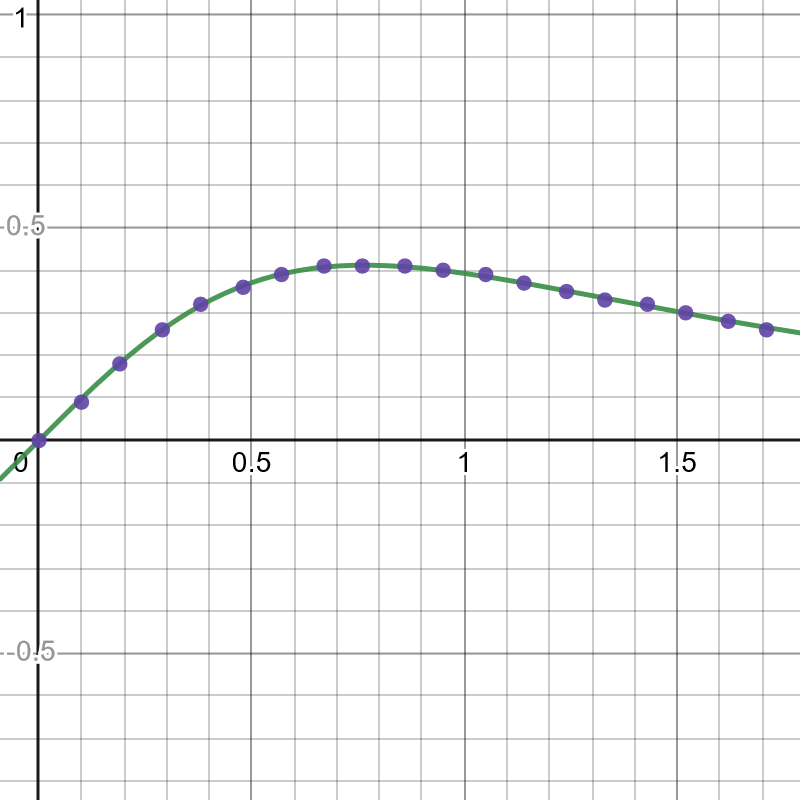
\includegraphics[scale=0.3]{src/least_sqr_des.png}
    \captionof{figure}{График аппроксимации МНК при $n=20, m = 12$}
\end{center}

\subsubsection*{Задача №4}
\begin{enumerate}
    \item Написать вычислительную программу на языке программирования C++
    для решения методом прогонки СЛАУ с 5-диагональной матрицей
    следующего вида:
    \begin{center}
        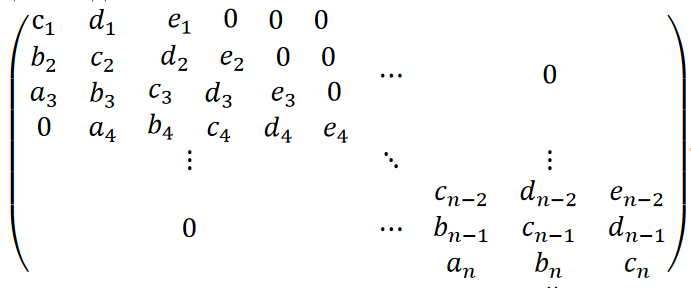
\includegraphics[]{src/pentadiagonal.png}
    \end{center}
    \item Для отладки программы написать генератор случайных вещественных
матриц данного вида с диагональным преобладанием.
\end{enumerate}
\subsubsection*{Решение}
Система записывается в следующем виде:
\begin{equation*}
    \begin{aligned}
        \qquad \qquad \qquad c_0y_0+d_0y_1+e_0y_2&=f_0 \\
        \qquad \quad b_1y_0+c_1y_1+d_1y_2+e_1y_3&=f_1 \\
        a_2y_{0}+b_2y_{1}+c_2y_{2}+d_2y_{3}+e_2y_{4}&=f_2\\
        \dots \\
        a_iy_{i-2}+b_iy_{i-1}+c_iy_{i}+d_iy_{i+1}+e_iy_{i+2}&=f_i\\
        \dots \\
        a_{n-3}y_{n-5}+b_{n-3}y_{n-4}+c_{n-3}y_{n-3}+d_{n-3}y_{n-2}+e_{n-3}y_{n-1}&=f_{n-3}\\
        a_{n-2}y_{n-4}+b_{n-2}y_{n-3}+c_{n-2}y_{n-2}+d_{n-2}y_{n-1}&=f_{n-2}\\
        a_{n-1}y_{n-3}+b_{n-1}y_{n-2}+c_{n-1}y_{n-1} &=f_{n-1}
    \end{aligned}
\end{equation*}
Выразим все $y_i$ в виде 
\begin{equation*}
    y_i=\alpha_iy_{i+1}+\beta_iy_{i+2}+\gamma_i
\end{equation*}
Тогда, 
\begin{equation*}
    \begin{aligned}
        z_0 &=c_0 \\
        \alpha_0&=\frac{-d_0}{z_0} \\
        \beta_0&=\frac{-e_0}{z_0} \\
        \gamma_0&=\frac{f_0}{z_0} \\
        z_1&=b_1\alpha_0+c_1 \\
        \alpha_1&=\frac{-(b_1\beta_0+d_1)}{z_1}\\
        \beta_1&=\frac{-e_1}{z_1}\\
        \gamma_1&=\frac{f_1-b_1\gamma_0}{z_1}\\
        i\in[2,n)\\
        z_i&=a_i\alpha_{i-2}\alpha_{i-1}+a_i\beta_{i-2}+b_i\alpha_{i-1}+c_i\\
        \alpha_i&=\frac{-(a_i\alpha_{i-2}\beta_{i-1}+b_i\beta_{i-1}+d_i)}{z_i}\\
        \beta_i&=\frac{-e_i}{z_i}\\
        \gamma_i&=\frac{f_i-(a_i\alpha_{i-2}\gamma_{i-1}+a_i\gamma_{i-2}+b_i\gamma_{i-1})}{z_i}\\
    \end{aligned}
\end{equation*}
Тогда можно выразить все $y_i$ в обратном порядке
\begin{equation*}
    \begin{aligned}
        y_{n-2}&=\alpha_{n-2}y_{n-1}+\gamma_{n-2}\\
        y_{n-1}&=\frac{f_{n-1}-(a_{n-1}\alpha_{n-3}\gamma_{n-2}+a_{n-1}\gamma_{n-3}+b_{n-1}\gamma_{n-2})}{a_{n-1}\alpha_{n-3}\alpha_{n-2}+a_{n-1}\beta_{n-3}+b_{n-1}\alpha_{n-2}+c_{n-1}}\\
        i\in[n-3,0]\\
        y_i&=\alpha_iy_{i+1}+\beta_iy_{i+2}+\gamma_i\\
        y_0 &=\frac{f_0-d_0y_1-e_0y_2}{c_0} \\
    \end{aligned}
\end{equation*}
\newpage
Для примера была сгенерирована система:

\begin{equation}
    \label{eq:pentadiagonal}
    \begin{pmatrix}
        7.00& 2.00& 8.00& 0.00& 0.00& 0.00& 0.00& 0.00&\\
        3.00&10.00& 5.00& 2.00& 0.00& 0.00& 0.00& 0.00&\\
        8.00& 2.00& 2.00& 3.00& 2.00& 0.00& 0.00& 0.00&\\
        0.00& 8.00&10.00& 7.00&10.00& 6.00& 0.00& 0.00&\\
        0.00& 0.00& 6.00&10.00&10.00&10.00& 1.00& 0.00&\\
        0.00& 0.00& 0.00& 8.00& 2.00& 3.00& 4.00& 3.00&\\
        0.00& 0.00& 0.00& 0.00& 4.00& 5.00& 2.00& 7.00&\\
        0.00& 0.00& 0.00& 0.00& 0.00& 8.00& 1.00& 4.00&
    \end{pmatrix}
    \begin{pmatrix}
       x_1\\x_2\\x_3\\x_4\\x_5\\x_6\\x_7\\x_8
    \end{pmatrix}
    =
    \begin{pmatrix}
        4.00\\  2.00\\  4.00\\  8.00\\ 10.00\\  5.00\\  2.00\\ 10.00\\
    \end{pmatrix}
\end{equation}

Вычисление системы \eqref{eq:pentadiagonal} пятидиагональной прогонкой даёт результат:
\begin{equation*}
    \begin{pmatrix}
       x_1\\x_2\\x_3\\x_4\\x_5\\x_6\\x_7\\x_8
    \end{pmatrix}
    =
    \begin{pmatrix}
        3.99\\  3.92\\ -3.97\\-14.67\\  8.10\\  6.33\\ 36.20\\-19.21\\
    \end{pmatrix}
\end{equation*}

Аналогичный результат получается при использовании пакета Maple. Скриншот ноутбука продемонстрирован на рисунке 4.

\begin{center}
    \label{maple}
        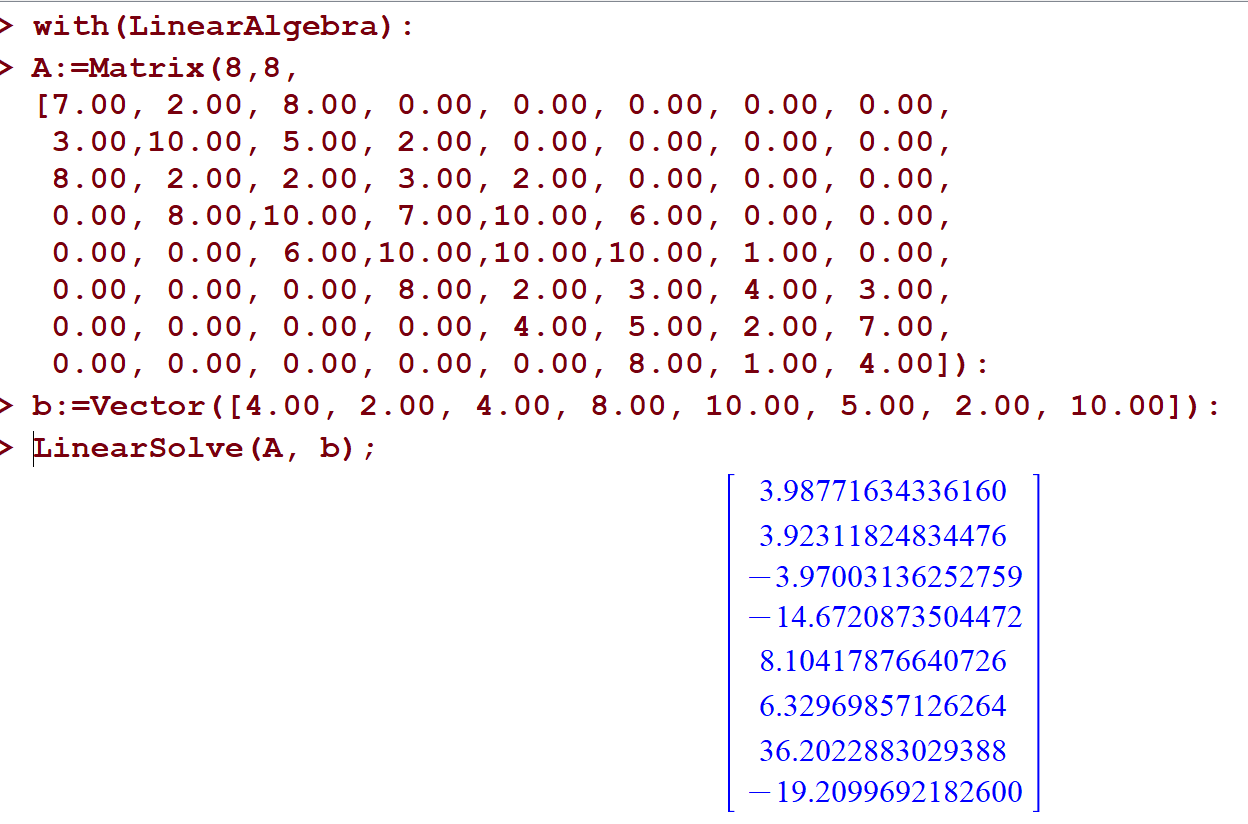
\includegraphics[scale=0.3]{src/maple_sol.png}
    \captionof{figure}{Скриншот программы Maple 19 с решением задачи \eqref{eq:pentadiagonal}}
\end{center}
\newpage
\subsection*{Вывод}
В результате проделанной лабораторной работы был изучен теоретический материал необходимый для решения поставленных задач по численному решению систем линейных алгебраических уравнений с использованием различных прямых методов и для каждой поставленной задачи написана вычислительная программа на языке программирования С++.
\newpage
\subsection*{Список литературы}
\begin{enumerate}
    \item Бахвалов Н.С., Жидков Н.П., Кобельков Г.М. Численные методы: Бином, 2018. – 636 с. 
    \item Калиткин Н.Н. Численные методы, 2-е издание: БХВ-Петербург, 2014. – 592 с.
    \item Самарский А.А., Гулин А. В. Численные методы: Учеб, пособие для вузов, — М.: Наука. Гл. ред. физ-мат. лит., 1989.— 432 с.
\end{enumerate}
\newpage
\subsection*{Приложение}
Весь код выложен в github-репозитории по ссылке: 

\url{https://github.com/sultanovMF/Numerical-Methods-Lab}

\end{document}


